% This is "sig-alternate.tex" V2.1 April 2013
% This file should be compiled with V2.5 of "sig-alternate.cls" May 2012
%
% This example file demonstrates the use of the 'sig-alternate.cls'
% V2.5 LaTeX2e document class file. It is for those submitting
% articles to ACM Conference Proceedings WHO DO NOT WISH TO
% STRICTLY ADHERE TO THE SIGS (PUBS-BOARD-ENDORSED) STYLE.
% The 'sig-alternate.cls' file will produce a similar-looking,
% albeit, 'tighter' paper resulting in, invariably, fewer pages.
%
% ----------------------------------------------------------------------------------------------------------------
% This .tex file (and associated .cls V2.5) produces:
%       1) The Permission Statement
%       2) The Conference (location) Info information
%       3) The Copyright Line with ACM data
%       4) NO page numbers
%
% as against the acm_proc_article-sp.cls file which
% DOES NOT produce 1) thru' 3) above.
%
% Using 'sig-alternate.cls' you have control, however, from within
% the source .tex file, over both the CopyrightYear
% (defaulted to 200X) and the ACM Copyright Data
% (defaulted to X-XXXXX-XX-X/XX/XX).
% e.g.
% \CopyrightYear{2007} will cause 2007 to appear in the copyright line.
% \crdata{0-12345-67-8/90/12} will cause 0-12345-67-8/90/12 to appear in the copyright line.
%
% ---------------------------------------------------------------------------------------------------------------
% This .tex source is an example which *does* use
% the .bib file (from which the .bbl file % is produced).
% REMEMBER HOWEVER: After having produced the .bbl file,
% and prior to final submission, you *NEED* to 'insert'
% your .bbl file into your source .tex file so as to provide
% ONE 'self-contained' source file.
%
% ================= IF YOU HAVE QUESTIONS =======================
% Questions regarding the SIGS styles, SIGS policies and
% procedures, Conferences etc. should be sent to
% Adrienne Griscti (griscti@acm.org)
%
% Technical questions _only_ to
% Gerald Murray (murray@hq.acm.org)
% ===============================================================
%
% For tracking purposes - this is V2.0 - May 2012

\documentclass{sig-alternate-05-2015}

\DeclareMathOperator*{\argmin}{arg\,min}
\usepackage{booktabs}
\usepackage{hyperref}

\begin{document}

% Copyright
\setcopyright{acmcopyright}
%\setcopyright{acmlicensed}
%\setcopyright{rightsretained}
%\setcopyright{usgov}
%\setcopyright{usgovmixed}
%\setcopyright{cagov}
%\setcopyright{cagovmixed}


% DOI
%\doi{10.475/123_4}

% ISBN
%\isbn{123-4567-24-567/08/06}

%Conference
%\conferenceinfo{PLDI '13}{June 16--19, 2013, Seattle, WA, USA}

%\acmPrice{\$15.00}

%
% --- Author Metadata here ---
%\conferenceinfo{WOODSTOCK}{'97 El Paso, Texas USA}
%\CopyrightYear{2007} % Allows default copyright year (20XX) to be over-ridden - IF NEED BE.
%\crdata{0-12345-67-8/90/01}  % Allows default copyright data (0-89791-88-6/97/05) to be over-ridden - IF NEED BE.
% --- End of Author Metadata ---

\title{On the Feasibility of Optimizing Software Product Lines with Quantum Annealing}

% You need the command \numberofauthors to handle the 'placement
% and alignment' of the authors beneath the title.
%
% For aesthetic reasons, we recommend 'three authors at a time'
% i.e. three 'name/affiliation blocks' be placed beneath the title.
%
% NOTE: You are NOT restricted in how many 'rows' of
% "name/affiliations" may appear. We just ask that you restrict
% the number of 'columns' to three.
%
% Because of the available 'opening page real-estate'
% we ask you to refrain from putting more than six authors
% (two rows with three columns) beneath the article title.
% More than six makes the first-page appear very cluttered indeed.
%
% Use the \alignauthor commands to handle the names
% and affiliations for an 'aesthetic maximum' of six authors.
% Add names, affiliations, addresses for
% the seventh etc. author(s) as the argument for the
% \additionalauthors command.
% These 'additional authors' will be output/set for you
% without further effort on your part as the last section in
% the body of your article BEFORE References or any Appendices.

\numberofauthors{2} %  in this sample file, there are a *total*
% of EIGHT authors. SIX appear on the 'first-page' (for formatting
% reasons) and the remaining two appear in the \additionalauthors section.
%
\author{
% You can go ahead and credit any number of authors here,
% e.g. one 'row of three' or two rows (consisting of one row of three
% and a second row of one, two or three).
%
% The command \alignauthor (no curly braces needed) should
% precede each author name, affiliation/snail-mail address and
% e-mail address. Additionally, tag each line of
% affiliation/address with \affaddr, and tag the
% e-mail address with \email.
%
% 1st. author
\alignauthor
Timothy Goodrich\\
\affaddr{Department of Computer Science}\\
\affaddr{North Carolina State University}\\
\affaddr{Raleigh, North Carolina 27606}\\
\email{tdgoodri@ncsu.edu}
}
\date{7 December 2016}
% Just remember to make sure that the TOTAL number of authors
% is the number that will appear on the first page PLUS the
% number that will appear in the \additionalauthors section.

\maketitle
\begin{abstract}
Software product lines are an abstract representation of real-world software engineering problems.
\end{abstract}

%
% %
% % The code below should be generated by the tool at
% % http://dl.acm.org/ccs.cfm
% % Please copy and paste the code instead of the example below.
% %
% \begin{CCSXML}
% <ccs2012>
%  <concept>
%   <concept_id>10010520.10010553.10010562</concept_id>
%   <concept_desc>Computer systems organization~Embedded systems</concept_desc>
%   <concept_significance>500</concept_significance>
%  </concept>
%  <concept>
%   <concept_id>10010520.10010575.10010755</concept_id>
%   <concept_desc>Computer systems organization~Redundancy</concept_desc>
%   <concept_significance>300</concept_significance>
%  </concept>
%  <concept>
%   <concept_id>10010520.10010553.10010554</concept_id>
%   <concept_desc>Computer systems organization~Robotics</concept_desc>
%   <concept_significance>100</concept_significance>
%  </concept>
%  <concept>
%   <concept_id>10003033.10003083.10003095</concept_id>
%   <concept_desc>Networks~Network reliability</concept_desc>
%   <concept_significance>100</concept_significance>
%  </concept>
% </ccs2012>
% \end{CCSXML}
%
% \ccsdesc[500]{Computer systems organization~Embedded systems}
% \ccsdesc[300]{Computer systems organization~Redundancy}
% \ccsdesc{Computer systems organization~Robotics}
% \ccsdesc[100]{Networks~Network reliability}


%
% End generated code
%

%
%  Use this command to print the description
% %
% \printccsdesc

% We no longer use \terms command
%\terms{Theory}

\keywords{Software Product Lines; Adiabatic Quantum Computing; Multi-Objective Optimization}

\section{Introduction}
\subsection{Motivation}
Many software engineering problems reduce to optimization. How can we efficiently generate effect tests? How can we tune learners to accurately predict for bugs? How can we optimize the features offered in a product? Each of these classic problems are typically formulated as optimization problems at the intersection of search-based software engineering \cite{harman2001search} and functional testing \cite{beizer1995black}, defect prediction \cite{fenton1999critique}, and product line optimization \cite{kang1990feature}, respectively. Unfortunately, these problems are nearly always NP-hard for an optimal solution and difficult to estimate, creating run times that hampered by exponential-sized search spaced. Developing fast, automated tools for solving these optimization problems, therefore, is of high practical interest to the software engineering community.

As mentioned above, one area of interest is Software Product Line (SPL) optimization (Figure \ref{figure:phone}). SPL models represent the full feature set of a product line. In the phone example, the different features such as GPS and screen density are listed, and specific phone instances (i.e. a specific phone product number) are found with valid configurations of the SPL model. For example, one valid cell phone can make calls, does not have a GPS, has a high resolution screen, and has a camera. Formally, SPLs are Constraint Satisfaction Problems, where a tree of features are connected with \emph{mandatory} and \emph{optional} edges, and \emph{alternative} or (multiple-allowed) \emph{or} children. Across this tree are \emph{cross-tree constraints}, denoting \emph{requirements} and \emph{exclusions}. For example, the GPS feature excludes having a basic screen (and vice versa), and the camera requires having a high resolution screen.

\begin{figure}[!h]
\centering
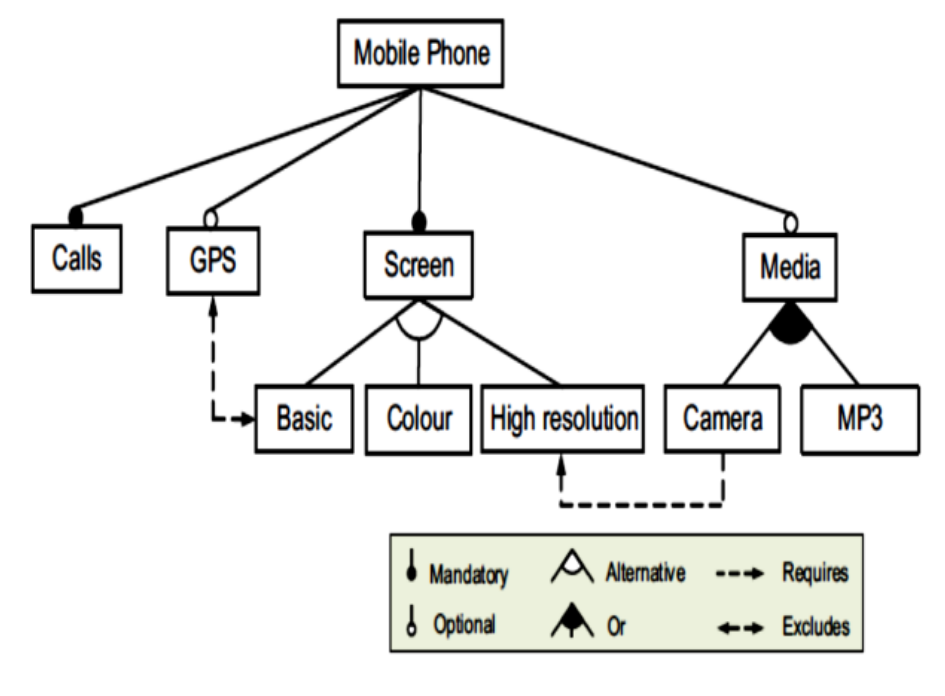
\includegraphics[width=0.48\textwidth]{images/phone}
\caption{The phone software product line from \cite{benavides2010automated}}
\label{figure:phone}
\end{figure}

While finding configurations to satisfy such a small, tree-like example is not hard, the problem becomes exponentially harder as the CSP becomes less and less tree-like. Specifically, CSPs are NP-hard using a trivial reduction of satisfiability (SAT). Therefore finding all valid configurations of a SPL model is considered difficult.

Compounding the complexity, usually more real-world information is provided with these models. Factors such as feature cost, feature reliability, and feature reception (i.e. tried-and-true measure) all provide different information and so must be solved using \emph{multi-objective optimization}. Such optimization methods typically imply genetic algorithms such as NSGA-II \cite{deb2002fast} and SPEA 2 \cite{chang2007sub}, but other optimization methods apply.

One such alternative is Chen et al.'s SWAY algorithm \cite{chen2016sampling}. The SWAY algorithm begins by using a SAT-solver to generate all valid configurations of a SPL model, then uses precise sampling to efficiently find Pareto-optimal solutions. The authors found that the SAT-solver is actually the computational bottleneck in practice. Note that using a SAT solver this way is naturally a serial operation: once an initial solution is found, the $i$th solution is found by solving the same formula \emph{and} the negation of the first $i-1$ solutions. With this approach restricted to serial operation, a scalable alternative is desirable.

In this paper, we introduce the notion of using \emph{quantum annealing} to find valid configurations of a SPL model. Based on the \emph{adiabatic quantum computing} model by Farhi et al. \cite{farhi2000quantum}, quantum annealing evolves an initial quantum system (represented by a Hamiltonian) to a final quantum system. The adiabatic theorem \cite{farhi2000quantum} guarantees that a slow-enough evolution leaves the final quantum system in a \emph{ground state}, therefore a state of minimum energy can be computed with the system if appropriate \emph{charges} are applied to the initial quantum system. Popularized by the D-Wave System Inc. production models, quantum annealing is rapidly becoming a viable alternative to optimization black boxes such as SAT-solvers.

\begin{figure}[!h]
\centering
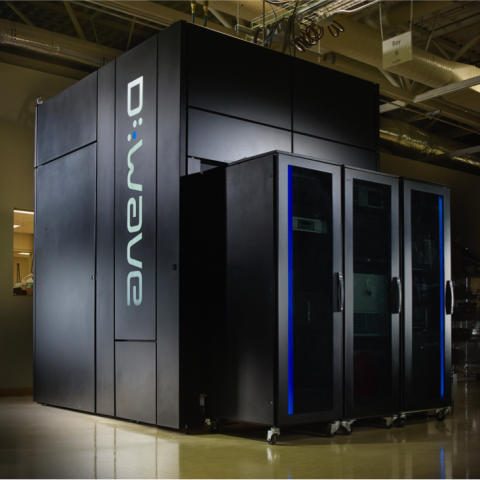
\includegraphics[width=0.48\textwidth]{images/dwave}
\caption{The D-Wave System Inc.'s \emph{D-Wave 2X} quantum annealer. The primary cooling unit houses a 1152-qubit processor, with IO and networking handled by a front-mounted server rack.}
\label{figure:dwave}
\end{figure}

The primary motivation to use a quantum annealer for SPL model optimization is for the \emph{quantum solutions}. In classical computing, an optimal solution to an optimization problem is an assignment such that an objective function is maximized or minimized (as desired). Several such optimal solutions can exist, of course. However, in quantum computing, an optimal solution is a \emph{uniform probability distribution} over all assignments that maximize or minimize the objective function. One effect of this nuance is that very rugged terrain in the objective function leads to faster solution convergence; the solution takes advantage of \emph{quantum tunneling} to burrow through objective function hills. The speedups from quantum tunneling have proven to be exponential, with work by \cite{denchev2015computational} showing a speedup of over 10,000,000 compared to classical annealing algorithms.

More useful for the SPL model optimization, though, is a second effect: a single run of the quantum annealer returns a distribution over the solutions found. These solutions are ranked by energy, which is a dependent function on the optimization problem's objective function, therefore optimal solutions are immediately recognizable. Given the standard run time of a modern D-Wave 2X annealer, over 1000 solutions can be collected in under a second. Again, given the serialization of SAT solvers for finding all valid configurations, the run times of this quantum annealer offer a reasonable alternative to classical algorithms, even in its experimental stage.

The downside to the quantum annealer is the amount of resources available, though. The current generation D-Wave 2X offers 1152-qubits in a \emph{Chimera} graph layout, which is very sparse in terms of connections between qubits. These connections provide the analog of ``memory'' when embedding an optimization problem, so in effect there are a very limited number of constraints possible per qubit. To overcome this problem, multiple qubits can be assigned to represent a single optimization problem variable, so then the bottleneck comes entirely from how many qubits the optimization problem requires.

\subsection{Contributions}
In this paper we set the groundwork for developing full-pipeline algorithms for embedding CSP (specifically SPL) optimization problems into the D-Wave 2X. Our goals are defined by the following research questions:

\begin{itemize}
\item \textbf{RQ1 (Available Methods):} \emph{What methods are there for converting SAT-based optimization problems into Ising Model problems?}
\item \textbf{RQ2 (Method Practicality):} \emph{How badly do these conversion methods blow up the initial problem?}
\item \textbf{RQ3 (Bottlenecks):} \emph{What problems can we expect to run on current hardware and expected future hardware? What problems are keeping larger problems from running?}
\end{itemize}

The remainder of this paper is organized as follows. Section provides background on related work in optimizing Software Product Lines, along with a general overview on how to use the D-Wave 2X quantum annealer. Section 3 outlines our work on developing algorithms for converting SPL datasets from the SPLOT repository into the \emph{Ising Model} format needed to communicate with the D-Wave 2X, and we provide an overview of the software developed for these algorithms. Section 4 summarizes our experimental results on the SPLOT datasets, and we offer observations the practical implications. Section 5 provides a summary of the results presented in this paper, a justification on the scientific nature of this work, an overview of planned additional work.

\section{Background}

\begin{figure*}[!h]
\centering
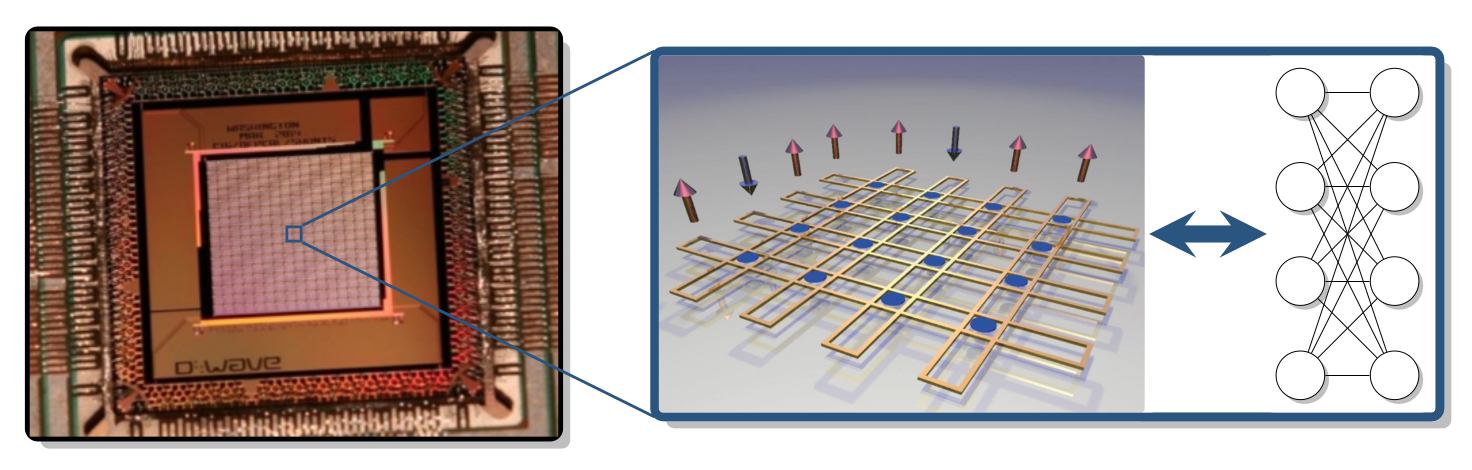
\includegraphics[width=0.98\textwidth]{images/hardware}
\caption{(Left) The D-Wave System Inc.'s upcoming \emph{D-Wave 2000Q} 2048-qubit processor, a $16 \times 16$ grid of cells; (Center) a single cell, where 4 qubits (long) are overlaid on 4 other qubits orthogonally, with 16 overlapping areas that are used for qubit couplers. (Right) The graph-theoretic interpretation of a cell: a complete bipartite graph $K_{4,4}$. From
\cite{goodrich2016graph}.}
\label{figure:hardware}
\end{figure*}

\subsection{Related Work}
Feature models were first introduced to software engineering by Kang et al. in the 1990s \cite{kang1990feature}. An excellent survey by Benavides et al. covers the last 20 years of approaches \cite{benavides2010automated}. They note that SAT solvers are by far the most common approach, with some alternatives being binary decision diagrams (BDDs) and Carnegie Mellon's SMV model checker.

In more recent years, several product-line--specific algorithms have been published, such as Sayyad et al.'s IBEASEED \cite{sayyad2013scalable} and Henard et al.'s SATIBEA \cite{henard2015combining}. The latter uses genetic algorithms to explore the (valid and invalid) solution space, and uses a SAT solver to patch together invalid solutions that resulted from mutation. We base our work off of the recent work by Chen et al. \cite{chen2016sampling}, who use a SAT solver to build the (valid) solution space first before doing multi-objective optimization.

In this context, we suggest the reader views quantum annealing as a black-box replacement for a SAT solver. As mentioned before, the quantum tunneling facet of the machine makes generating multiple solutions an advantage over a standard SAT solver, but this advantage could be used in other ways. For example, a majority of solutions could be generated by quantum annealing, following by using a SAT solver to solve the (reduced) formula exactly for the remaining few solutions. Alternately, some solutions in the quantum annealing distribution might not be valid, but rather a fairly-optimal solution to the MAX-SAT version of the problem. In this case we could view these solutions as mutations with a high number of satisfied clauses, and generate these mutations as a middle step in a modified version of Henard et al.'s SATIBEA algorithm.

\subsection{D-Wave Quantum Annealing}

Adiabatic quantum computing was first published about in the early 2000s by Farhi et al. \cite{farhi2000quantum}. The model was introduced as an alternative to the \emph{circuit-based quantum computing} model that has dominated the literature. Theoretically, the two models are equivalent, and equivalent also to the \emph{universal quantum computer}, an analog to the Turing Machine for quantum computing.

In 2011, D-Wave Systems Inc. produced their first production-quality quantum annealer, the 128-qubit D-Wave One. Based on adiabatic quantum computing, the quantum annealer is fundamentally limited by physical constraints and \emph{not} equivalent to the universal quantum computer. However, the annealer excels at solving a quantum mechanics problem, the \emph{Ising Model problem}:

\begin{equation}
\label{eq:ising}
    \displaystyle \argmin \sum_{1 \leq i \leq n} a_i s_i + \sum_{i < j} b_{ij} s_i s_j
\end{equation}

where $a_i, b_{ij} \in \mathbb{R}$ and $s_i \in \{-1, +1\}$. The $s_i$ variables are the qubits and are assigned \emph{spins}. This equation is naturally represented as a graph with vertices $s_i$, edges $s_i s_j$, vertex weights $a_i$ and edge weights $b_{ij}$. Figure \ref{figure:hardware} visualizes an upcoming D-Wave chip, the qubits, and the graph form.

\begin{figure*}[!h]
\centering
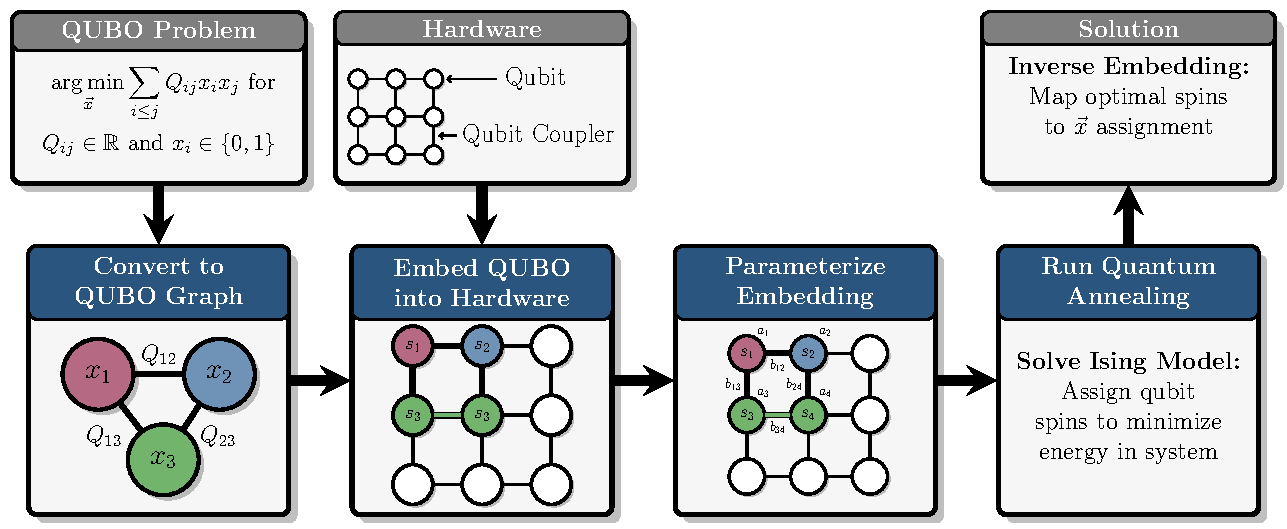
\includegraphics[width=0.98\textwidth]{images/pipeline}
\caption{The algorithmic pipeline for embedding a QUBO into an Ising Model, running the hardware, and mapping the quantum solution back to the original optimization problem. From \cite{goodrich2016graph}.}
\label{figure:pipeline}
\end{figure*}

One limitation of the D-Wave hardware vs. the theoretical quantum annealing model is that not all possible edges are present in the D-Wave hardware. The D-Wave hardware has classically been instances of \emph{Chimera} graphs, an $M \times N$ grid of complete bipartite cells (Figure \ref{figure:hardware}). To circumvent this issue, Choi \cite{choi2011minor} introduced the notion of \emph{minor embedding} an optimization problem graph into the hardware graph. At a high level, minor embedding selects a connected set of \emph{physical qubits} from the hardware graph to represent each \emph{logical qubit} in the problem graph. The vertex and edge weights from the problem graph are then
distributed appropriately onto the physical qubits, providing a mapping between the \emph{Ising Model} version of the problem that the quantum annealer solves and the optimization problem that the user is interested in solving. Figure \ref{figure:pipeline} visualizes this process.

We note that optimization problems are typically formulated as \emph{quadratic unconstrained binary optimization problems (QUBOs)}, defined as the following:

\begin{equation}
\label{eq:qubo}
    \displaystyle \argmin \sum_{i < j} c_{ij} x_i x_j
\end{equation}

where $c_{ij} \in \mathbb{R}$ and $x_i \in \{0, 1\}$. Note how similar Equations \ref{eq:ising} and \ref{eq:qubo} are, a simple variable change can convert from one to the other. We recommend the analogy of a QUBO is to quantum annealing what a linear program is to an LP-solver -- each are formats for feeding optimization problems into tuned black boxes.

Unfortunately, minor embedding is itself an NP-hard problem, and Choi mentions that previous algorithms for distributing logical processes on physical nodes from parallel computing do not apply. However, in the last five years several papers have been published with embedding algorithms to handle different structural considerations \cite{boothby2016fast, goodrich2016graph, klymko2014adiabatic}, and D-Wave provides an in-house heuristic in their API \cite{cai2014practical}.

In total, the D-Wave quantum annealer has experienced rapid improvements over the last five years. The first iteration, the D-Wave One, was a $4 \times 4$ grid of $K_{4,4}$ cells. The next two models, the D-Wave Two and 2X, upped the grid sizes to $8 \times 8$ and $12 \times 12$, respectively. The D-Wave 2X is actually a partially-disabled $16 \times 16$ grid, and a more mature manufacturing process is currently under development to yield the next generation $2048$-qubit D-Wave $2000Q$ model.

In terms of performance and applications, a recent paper by the research group at Google, one of the primary clients, showed a problem with a harsh energy landscape that the D-Wave annealer could solve 10,000,000 times faster than classical approaches \cite{denchev2015computational}. Major applications also exist in computational chemistry \cite{kassal2010simulating}, image recognition \cite{neven2008image}, NASA Mars missions \cite{venturelli2015quantum}, and Karp's 21 NP-hard problems \cite{lucas2013ising}.


\section{RQ1: Available Methods}

In the last section we saw how much of the D-Wave embedding research effort has assumed that an optimization problem is provided as a QUBO, which can then be embedded into the hardware's Ising Model. Therefore the first step to running Software Product Line optimization on the quantum annealer is to obtain a QUBO formulation. In this section we explore different ways of accomplishing this conversion. While none of these algorithms are spelled out explicitly, we use a few conversion techniques are used D-Wave documentation \cite{dwave}.

\subsection{Method 1: Maximum Independent Set}
\begin{figure}[!h]
\centering
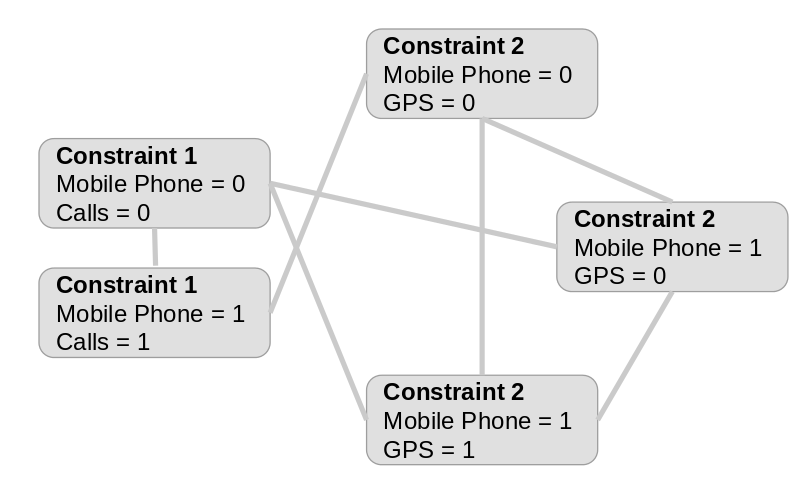
\includegraphics[width=0.48\textwidth]{images/mis}
\caption{A conflict graph for two constraints: Mobile Phone $\longleftrightarrow$ Calls and GPS $\to$ Mobile Phone}
\label{figure:mis}
\end{figure}

\begin{table*}[!h]
\centering
\begin{tabular}{l l}
\toprule
Constraint & Penalty\\
\midrule
$z \iff \neg x$ & $2xz - x - z + 1$\\
$z \iff x_1 \lor x_2$ & $x_1 x_2 + (x_1 + x_2)(1-2z)+z$\\
$z \iff x_1 \land x_2$ & $x_1 x_2 - 2(x_1 + x_2)z + 3z$\\
$z \iff x_1 \oplus x_2$ & $2x_1x_2 - 2(x_1 + x_2)z - 4(x_1 + x_2)a + 4az + x_1 + x_2 + z + 4a$\\
\bottomrule
\end{tabular}
\label{table:gadgets}
\caption{Boolean logic as penalty-based posiforms.}
\end{table*}

The first method we will outline is based on solving a maximum independent set (MIS) problem. The algorithm first converts the SPL dataset into a satisfiability problem with any first-order logical operator (and, or, not, if, iff). Then a \emph{conflict graph} (Figure \ref{figure:mis}) is constructed, where vertices are valid assignments to the SPL features and there is an edge between two vertices if they conflict on an assignment. For example, given the constraint \textbf{Mobile Phone} $\longleftrightarrow$ \textbf{Calls}, which corresponds to the ``mandatory'' edge from the SPL, there are two valid assignments: either both features are zero or both are one. For the constraint \textbf{GPS} $\to$ \textbf{Mobile Phone} (i.e. the GPS is optional) there are three valid assignments: everything is zero, everything is one, and the phone is one while the GPS is zero. These assignments generate the vertices of the
graph and edges denote where assignments have conflicts. For example, we cannot set \textbf{Mobile Phone}$~=~0$, \textbf{Calls}$~=~0$ and \textbf{Mobile Phone}$~=~1$, \textbf{GPS}$~=~0$. While both assignments are valid individually, they disagree on \textbf{Mobile Phone}, and so are not a valid global assignment. Therefore there is an edge between these two assignments in the conflict graph.

Once the conflict graph is constructed, we find a valid assignment if and only if we can find an independent set of size equal to the number of constraints in the SPL model. In graph theory, in independent set is a set of vertices such that no two vertices have an edge between them. In this problem, an independent set says that we have found an assignment that does not have any conflicts, and we satisfy one constraint from the SPL model for each vertex in our independent set. Given that any two vertices for a single constraint will have an edge between them (i.e. they are two distinct assignments), we know that a maximum independent set will satisfy all constraints, therefore a solution to this problem will satisfy the SLP model.


At first glance, choosing maximum independence set as a format seems like a poor choose, given that it is classically NP-hard. However, an early result from Choi \cite{choi2011minor} showed that MIS has a \emph{posiform} formulation compatible with QUBOs:

\begin{equation}
\min_{x} \left\{ \sum_{v \in V} \bar{x}_v + M \sum_{v,v' \in E} x_v x_{v'} \right\}
\end{equation}

where $x_v \in \{0, 1\}$ and $M \in \mathbb{R}^+$ is a penalty constant. Note what this equation is saying at a high-level: minimize this equation where $\bar{x}$ (not $x$) is minimized (i.e. the number of vertices is maximized), and the number of occurrences of $x_v = x_{v'} = 1$ with a multiplied penalty is minimized (i.e. there is a penalty for every edge in the independent set). Therefore an optimal solution to this equation maximizes vertices and minimizes edges, and is an independent set. This posiform is in the QUBO format after replacing $\bar{x}$ with $(1-x)$.

In summary, this method converts SPL to a MIS instance, which then has a trivial conversion to a posiform, which then has a trivial conversion to a QUBO. In some sense this is the most efficient algorithm because we did not require the SPL model in any particular form, we just needed to derive the valid assignments. However, this assumption also makes this algorithm a poor choice in practice: each constraint forms a clique (a complete graph with all edges turned on). If a single constraint has several literals ``OR''ed together then the clique is exponential in the number of literals in the constraint. This is a particular problem for the Chimera graph because Klymko et al. \cite{klymko2014adiabatic} show with a treewidth argument that the Chimera graph can only embed cliques of up $LN+1$ (the cell height and the smallest grid dimension). Therefore these complete graphs will render the generated QUBO un-embeddable.

\subsection{Method 2: MAX-2-SAT Posiforms}
To combat the problem from the last method (exponential-sized cliques), we developed a second method using another posiform that converts easily to a QUBO: MAX-2-SAT. Recall that SLP models are typically expressed as Constraint Satisfiability Problems (CSPs), which are a type of satisfiability problem (SAT). Another variation of SAT is MAX-2-SAT, where clauses have at most two literals and each comes with a weight, and the goal is to maximize the sum of the weights from satisfied clauses. While 2-SAT is in P, the maximization part makes MAX-2-SAT NP-hard. Formulated as a posiform:

\begin{equation}
\min_{\vec{x}} \sum_c w_c \bar{l}_{c,1} \bar{l}_{c,2}
\end{equation}

where $w_c$ is the clause's weight and $l_{c,1}$ and $l_{c,2}$ are the literals. Note that the literals are negated in the posiform, meaning that we want to minimize the number of unsatisfied clauses.

Using this new posiform as the base of our conversion algorithm, the formulations we need are as follows. First, we convert the SLP model into a Conjunctive Normal Form version of SAT (uses only ``OR'' and ``NOT''). From CNF we use the gadgets from \ref{table:gadgets} to convert the problem to a MAX-SAT posiform, then conclude by converting the MAX-SAT posiform to a MAX-2-SAT posiform. What this means is that clauses with more than two literals need to be broken up by introducing auxiliary variables. Specifically, we need the following penalty function:

\begin{equation}
\label{eq:hubo}
x_1x_2x_3 = \min_z \left\{ zx_3 + M P(x_1, x_2; z))\right\}
\end{equation}

where

\begin{equation}
\label{eq:penalty}
P(x_1, x_2; z) = x_1x_2 - 2(x_1 + x_2)z + 3z.
\end{equation}

At a high level, Equation \ref{eq:hubo} says that we can introduce an auxiliary variable $z$ that represents $x_1x_2$, and it suffices to minimize $zx_3$ subject to a penalty if $x_1x_2$ does not agree with $z$. Equation \ref{eq:penalty} then is the gadget that links $z$ with $x_1x_2$, taken straight from Table \ref{table:gadgets}.

Note that the above gadget reduces a clause by one variable by introducing a new variable to represent two old ones, therefore the most efficient use of this gadget is in a binary tree. For example, for $x_1 x_2  x_3  x_4 x_5$ we would introduce $z_1$ to represent $x_1 x_2$, $z_2$ to represent $x_3 x_4$, $z_3$ to represent $z_1 z_2$, and we would then evaluate $x_5 z_3$.

In total, then, this method works by converting CSP to CNF, CNF to MAX-SAT posiform, MAX-SAT posiform to MAX-2-SAT posiform, then MAX-2-SAT posiform to QUBO using the same trivial change of variable used in the last method.

\subsection{Summary}

In summary, in this section we provide two methods for converting SPL model optimization problems into QUBOs. The first method utilizes maximum independent sets and required few conversions, but suffers from exponential-sized cliques. The second method requires many more conversions, but ultimately can handle the previously-problematic area (large ``OR'' clauses) with only a linear number of added constraints. In the next section we evaluate how this second method performs in practice.


\section{RQ2: Method Practicality}

In this section we evaluate the second method from the previous section. Specifically, we are interested in gauging if this conversion causes too much variable/constraint blowup for the method to be practical on the current hardware. Additionally, we are interested in looking at the graph structure in the generated QUBO, such that tuned minor embedding algorithms can take advantage of the structure.

\subsection{Data}
For data, we use the Software Product Line data available from the Software Product Lines Online Tools (SPLOT) repository (\url{http://www.splot-research.org/}). Table \ref{table:splot} lists the specific datasets we selected.

\begin{table*}[!h]
\centering
\begin{tabular}{l c c c c c c}
\toprule
Dataset Name & Features & \# Mandatory & \# Optional & \# XOR & \# OR & \# Cross-Tree Constraints\\
\midrule
Mobile Phone & 10 & 2 & 2 & 1 & 1 & 2\\
Webshop & 46 & 10 & 29 & 1 & 1 & 3\\
DELL Laptop/Notebook Computers & 47 & 7 & 1 & 8 & 0 & 38\\
BankingSoftware & 176 & 46 & 77 & 10 & 6 & 4\\
Electronic Shopping & 290 & 75 & 82 & 0 & 40 & 21\\
\bottomrule
\end{tabular}
\label{table:splot}
\caption{SPLOT datasets used.}
\end{table*}


\begin{table*}[!h]
\centering
\begin{tabular}{l c c c c c c}
\toprule
Dataset Name & Vertices & Edges & Diameter\\
\midrule
Mobile Phone & 17 & 22 & 5\\
Webshop & 52 & 63 & 8\\
DELL Laptop/Notebook Computers & 175 & 280 & 6\\
BankingSoftware & 243 & 300 & 11\\
Electronic Shopping & 323 & 331 & $\infty$\\
\bottomrule
\end{tabular}
\label{table:results}
\caption{Graph statistics for the QUBO generated by method 2 for each SPLOT dataset.}
\end{table*}

\subsection{Algorithm Implementation}
We provide the source code for the implementation of method 2 at \url{https://github.com/tdgoodrich/fss16tdg/tree/master/project/Code}.

\subsection{Experimental Results}

\subsection{Discussion}
Answer RQ1 by providing the best practice. Provide the following open problems: alternative formulation algorithms we could try (if any exist), different preprocessing techniques we could try (clustering, etc.), and directions for future algorithm design.

\section{Conclusion}

\subsection{Summary of Results}

\subsection{Validity of Software Science}
Why is this software science and not merely data dabbling?
\begin{itemize}
\item We asked and addressed concrete questions: We identify a best practice for converting SPL datasets into a D-Wave compatible format (RQ1), we see if D-Wave is currently a viable alternative to a SAT solver (RQ2), and see if D-Wave is worth using for large datasets (RQ3).
\item We used publicly-available and previously cited datasets.
\item We provide the output data from the D-Wave annealer (if we can, check with D-Wave).
\item We provide the scripts, configuration files, algorithm implementations for all experiments, along with a tutorial in the github repo on how to use these tools.
\item We provide conclusions that are based on tried-and-true statistical tests (Scott-Knot).
\end{itemize}

\subsection{Future Work}



\section{Acknowledgments}
Thank you to Professor Tim Menzies for his advice and support in the Foundations of Software Science course, and to Dr. Travis Humble for introduce the author to quantum annealing.

\newpage
\bibliographystyle{abbrv}
\bibliography{bib}  % sigproc.bib is the name of the Bibliography in this case

\end{document}
